%!TEX TS-program = xelatex

% Шаблон документа LaTeX создан в 2018 году
% Алексеем Подчезерцевым
% В качестве исходных использованы шаблоны
% 	Данилом Фёдоровых (danil@fedorovykh.ru) 
%		https://www.writelatex.com/coursera/latex/5.2.2
%	LaTeX-шаблон для русской кандидатской диссертации и её автореферата.
%		https://github.com/AndreyAkinshin/Russian-Phd-LaTeX-Dissertation-Template

\documentclass[a4paper,14pt]{article}


%%% Работа с русским языком
\usepackage[english,russian]{babel}   %% загружает пакет многоязыковой вёрстки
\usepackage{fontspec}      %% подготавливает загрузку шрифтов Open Type, True Type и др.
\defaultfontfeatures{Ligatures={TeX},Renderer=Basic}  %% свойства шрифтов по умолчанию
\setmainfont[Ligatures={TeX,Historic}]{Times New Roman} %% задаёт основной шрифт документа
\setsansfont{Comic Sans MS}                    %% задаёт шрифт без засечек
\setmonofont{Courier New}
\usepackage{indentfirst}
\frenchspacing

\renewcommand{\epsilon}{\ensuremath{\varepsilon}}
\renewcommand{\phi}{\ensuremath{\varphi}}
\renewcommand{\kappa}{\ensuremath{\varkappa}}
\renewcommand{\le}{\ensuremath{\leqslant}}
\renewcommand{\leq}{\ensuremath{\leqslant}}
\renewcommand{\ge}{\ensuremath{\geqslant}}
\renewcommand{\geq}{\ensuremath{\geqslant}}
\renewcommand{\emptyset}{\varnothing}

%%% Дополнительная работа с математикой
\usepackage{amsmath,amsfonts,amssymb,amsthm,mathtools} % AMS
\usepackage{icomma} % "Умная" запятая: $0,2$ --- число, $0, 2$ --- перечисление

%% Номера формул
%\mathtoolsset{showonlyrefs=true} % Показывать номера только у тех формул, на которые есть \eqref{} в тексте.
%\usepackage{leqno} % Нумерация формул слева	

%% Перенос знаков в формулах (по Львовскому)
\newcommand*{\hm}[1]{#1\nobreak\discretionary{}
	{\hbox{$\mathsurround=0pt #1$}}{}}

%%% Работа с картинками
\usepackage{graphicx}  % Для вставки рисунков
\graphicspath{{images/}}  % папки с картинками
\setlength\fboxsep{3pt} % Отступ рамки \fbox{} от рисунка
\setlength\fboxrule{1pt} % Толщина линий рамки \fbox{}
\usepackage{wrapfig} % Обтекание рисунков текстом

%%% Работа с таблицами
\usepackage{array,tabularx,tabulary,booktabs} % Дополнительная работа с таблицами
\usepackage{longtable}  % Длинные таблицы
\usepackage{multirow} % Слияние строк в таблице
\usepackage{float}% http://ctan.org/pkg/float

%%% Программирование
\usepackage{etoolbox} % логические операторы


%%% Страница
\usepackage{extsizes} % Возможность сделать 14-й шрифт
\usepackage{geometry} % Простой способ задавать поля
\geometry{top=20mm}
\geometry{bottom=20mm}
\geometry{left=20mm}
\geometry{right=10mm}
%
%\usepackage{fancyhdr} % Колонтитулы
% 	\pagestyle{fancy}
%\renewcommand{\headrulewidth}{0pt}  % Толщина линейки, отчеркивающей верхний колонтитул
% 	\lfoot{Нижний левый}
% 	\rfoot{Нижний правый}
% 	\rhead{Верхний правый}
% 	\chead{Верхний в центре}
% 	\lhead{Верхний левый}
%	\cfoot{Нижний в центре} % По умолчанию здесь номер страницы

\usepackage{setspace} % Интерлиньяж
\onehalfspacing % Интерлиньяж 1.5
%\doublespacing % Интерлиньяж 2
%\singlespacing % Интерлиньяж 1

\usepackage{lastpage} % Узнать, сколько всего страниц в документе.

\usepackage{soul} % Модификаторы начертания

\usepackage{hyperref}
\usepackage[usenames,dvipsnames,svgnames,table,rgb]{xcolor}
\hypersetup{				% Гиперссылки
	unicode=true,           % русские буквы в раздела PDF
	pdftitle={Практическая по БД},   % Заголовок
	pdfauthor={Подчезерцев Алексей},      % Автор
	pdfsubject={Создание и заполнение отношений БД фитнес-клуба},      % Тема
	pdfcreator={Подчезерцев Алексей}, % Создатель
	pdfproducer={Подчезерцев Алексей}, % Производитель
	pdfkeywords={БД} {SQL} {MySQL}, % Ключевые слова
	colorlinks=true,       	% false: ссылки в рамках; true: цветные ссылки
	linkcolor=black,          % внутренние ссылки
	citecolor=black,        % на библиографию
	filecolor=magenta,      % на файлы
	urlcolor=black           % на URL
}
\makeatletter 
\def\@biblabel#1{#1. } 
\makeatother
\usepackage{cite} % Работа с библиографией
%\usepackage[superscript]{cite} % Ссылки в верхних индексах
%\usepackage[nocompress]{cite} % 
\usepackage{csquotes} % Еще инструменты для ссылок

\usepackage{multicol} % Несколько колонок

\usepackage{tikz} % Работа с графикой
\usepackage{pgfplots}
\usepackage{pgfplotstable}

% ГОСТ заголовки
\usepackage[font=small]{caption}
%\captionsetup[table]{justification=centering, labelsep = newline} % Таблицы по правобу краю
%\captionsetup[figure]{justification=centering} % Картинки по центру


\newcommand{\tablecaption}[1]{\addtocounter{table}{1}\small \begin{flushright}\tablename \ \thetable\end{flushright}%	
\begin{center}#1\end{center}}

\newcommand{\imref}[1]{Рис.~\ref{#1}}

\usepackage{multirow}
\usepackage{spreadtab}
\newcolumntype{K}[1]{@{}>{\centering\arraybackslash}p{#1cm}@{}}


\usepackage{xparse}
\ExplSyntaxOn
\DeclareExpandableDocumentCommand{\juliandate}{ m m m }
{
	\juliandate_calc:nnnn { #1 } { #2 } { #3 } { \use:n }
}
\NewDocumentCommand{\storejuliandate}{ s m m m m }
{
	\IfBooleanTF{#1}
	{
		\juliandate_calc:nnnn { #3 } { #4 } { #5 } { \cs_set:Npx #2 }
	}
	{
		\juliandate_calc:nnnn { #3 } { #4 } { #5 } { \cs_new:Npx #2 }
	}
}
\cs_new:Npn \juliandate_calc:nnnn #1 #2 #3 #4 % #1 = day, #2 = month, #3 = year, #4 = what to do
{
	#4 
	{
		\int_eval:n
		{
			#1 +
			\int_div_truncate:nn { 153 * (#2 + 12 * \int_div_truncate:nn { 14 - #2 } { 12 } - 3) + 2 } { 5 } +
			365 * (#3 + 4800 - \int_div_truncate:nn { 14 - #2 } { 12 } ) +
			\int_div_truncate:nn { #3 + 4800 - \int_div_truncate:nn { 14 - #2 } { 12 } } { 4 } -
			\int_div_truncate:nn { #3 + 4800 - \int_div_truncate:nn { 14 - #2 } { 12 } } { 100 } + 
			\int_div_truncate:nn { #3 + 4800 - \int_div_truncate:nn { 14 - #2 } { 12 } } { 400 } -
			32045
		}
	}
}

\tl_new:N \l__juliandate_g_tl
\tl_new:N \l__juliandate_dg_tl
\tl_new:N \l__juliandate_c_tl
\tl_new:N \l__juliandate_dc_tl
\tl_new:N \l__juliandate_b_tl
\tl_new:N \l__juliandate_db_tl
\tl_new:N \l__juliandate_a_tl
\tl_new:N \l__juliandate_da_tl
\tl_new:N \l__juliandate_y_tl
\tl_new:N \l__juliandate_m_tl
\tl_new:N \l__juliandate_d_tl
\int_new:N \l_juliandate_day_int
\int_new:N \l_juliandate_month_int
\int_new:N \l_juliandate_year_int

\cs_new:Npn \__juliandate_set:nn #1 #2
{
	\tl_set:cx { l__juliandate_#1_tl } { \int_eval:n { #2 } }
}
\cs_new:Npn \__juliandate_use:n #1
{
	\tl_use:c { l__juliandate_#1_tl }
}
\cs_new_protected:Npn \juliandate_reverse:n #1
{
	\__juliandate_set:nn { g }
	{ \int_div_truncate:nn { #1 + 32044 } { 146097 } }
	\__juliandate_set:nn { dg }
	{ \int_mod:nn { #1 + 32044 } { 146097 } }
	\__juliandate_set:nn { c }
	{ \int_div_truncate:nn { ( \int_div_truncate:nn { \__juliandate_use:n { dg } } { 36524 } + 1) * 3 } { 4 } }
	\__juliandate_set:nn { dc }
	{ \__juliandate_use:n { dg } - \__juliandate_use:n { c } * 36524 }
	\__juliandate_set:nn { b }
	{ \int_div_truncate:nn { \__juliandate_use:n { dc } } { 1461 } }
	\__juliandate_set:nn { db }
	{ \int_mod:nn { \__juliandate_use:n { dc } } { 1461 } }
	\__juliandate_set:nn { a }
	{ \int_div_truncate:nn { ( \int_div_truncate:nn { \__juliandate_use:n { db } } { 365 } + 1) * 3 } { 4 } }
	\__juliandate_set:nn { da }
	{ \__juliandate_use:n { db } - \__juliandate_use:n { a } * 365 }
	\__juliandate_set:nn { y }
	{
		\__juliandate_use:n { g } * 400 + 
		\__juliandate_use:n { c } * 100 + 
		\__juliandate_use:n { b } * 4 + 
		\__juliandate_use:n { a }
	}
	\__juliandate_set:nn { m }
	{ \int_div_truncate:nn { \__juliandate_use:n { da } * 5 + 308 } { 153 } - 2 }
	\__juliandate_set:nn { d }
	{ \__juliandate_use:n { da } - \int_div_truncate:nn { (\__juliandate_use:n { m } + 4) * 153 } { 5 } + 122 }
	\int_set:Nn \l_juliandate_year_int
	{ \__juliandate_use:n { y } - 4800 + \int_div_truncate:nn { \__juliandate_use:n { m } + 2 } { 12 } }
	\int_set:Nn \l_juliandate_month_int
	{ \int_mod:nn { \__juliandate_use:n { m } + 2 } { 12 } + 1 }
	\int_set:Nn \l_juliandate_day_int
	{ \__juliandate_use:n { d } + 1 }
}
\cs_generate_variant:Nn \juliandate_reverse:n { x }

\NewDocumentCommand{\showday}{ m }
{
	\juliandate_reverse:n { #1 }
	\int_to_arabic:n { \l_juliandate_day_int }-
	\int_to_arabic:n { \l_juliandate_month_int }-
	\int_to_arabic:n { \l_juliandate_year_int }
}

\NewDocumentCommand{\tomorrow}{ }
{
	\group_begin:
	\juliandate_reverse:x { \juliandate_calc:nnnn { \day + 1 } { \month } { \year } { \use:n } }
	\day = \l_juliandate_day_int
	\month = \l_juliandate_month_int
	\year = \l_juliandate_year_int
	\today
	\group_end:
}
\NewDocumentCommand{\tomorrowof}{ m m m }
{
	\group_begin:
	\juliandate_reverse:x { \juliandate_calc:nnnn { #1 + 1 } { #2 } { #3 } { \use:n } }
	\day = \l_juliandate_day_int
	\month = \l_juliandate_month_int
	\year = \l_juliandate_year_int
	\today
	\group_end:
}
\ExplSyntaxOff


\usepackage{xcolor,listings}
\usepackage{textcomp}
\begin{document} % конец преамбулы, начало документа
\begin{titlepage}
	\begin{center}
		ФЕДЕРАЛЬНОЕ  ГОСУДАРСТВЕННОЕ АВТОНОМНОЕ \\
		ОБРАЗОВАТЕЛЬНОЕ УЧРЕЖДЕНИЕ ВЫСШЕГО ОБРАЗОВАНИЯ\\
		«НАЦИОНАЛЬНЫЙ ИССЛЕДОВАТЕЛЬСКИЙ УНИВЕРСИТЕТ\\
		«ВЫСШАЯ ШКОЛА ЭКОНОМИКИ»
	\end{center}
	
	\begin{center}
		\textbf{Московский институт электроники и математики}
		
		\textbf{Им. А.Н.Тихонова НИУ ВШЭ}
		
		\textbf{Департамент электронной инженерии}
	\end{center}	
	\vspace{5ex}
	\begin{center}
\textbf{<<ПОЛУЧЕНИЕ, ОБРАБОТКА И ПРЕДСТАВЛЕНИЕ РЕЗУЛЬТАТОВ МНОГОКРАТНЫХ ИЗМЕРЕНИЙ>>}
	\end{center}	
	\vspace{1ex}
	\begin{center}
\textbf{Отчёт по части 2 лабораторного практикума по дисциплине \\
	<<Электротехника, электроника и метрология>>, раздел <<Метрология>>(ЛР 5-7)}
	\end{center}	
	\vspace{5ex}
	
	\begin{multicols}{2}
	\vfill\null
	\columnbreak
	ВЫПОЛНИЛИ:
	
	Подчезерцев Алексей Евгеньевич
	
	Солодянкин Андрей Александрович
	
	группа БИВ172
	\end{multicols}

	\vfill
	\begin{center}
		Москва \the\year
	\end{center}
\end{titlepage}
\tableofcontents
\pagebreak

\section{ЦЕЛИ РАБОТЫ}
Целями данной работы являются:

\begin{itemize}
	\item получение навыков получения, обработки и представления результатов многократных измерений;
	\item формирование базовых навыков работы в среде NI LabVIEW по раз-работке компонентов для автоматизированной обработки результатов однократных измерений.
\end{itemize}

\section{ПРИМЕНЯЕМОЕ ОБОРУДОВАНИЕ И ПРОГРАММНОЕ ОБЕСПЕЧЕНИЕ}

\begin{enumerate}
	\item	Персональный компьютер (ПК).
	\item	Плата сбора данных NI-DAQ M-series PCI-6221/6251.
	\item	Кабель NI SH68-68-EPM Shielded Cable.
	\item	Коннекторный блок NI BNC 2120 
	\item	Провод соединительный коаксиальный (BNC-BNC).
	\item	Среда разработки NI LabVIEW 2013 Professional.
\end{enumerate}


\section{СТРУКТУРА ПРИКЛАДНОГО 	ПРОГРАММНОГО ОБЕСПЕЧЕНИЯ}
\subsection{Виртуальный прибор сбора и визуализации данных}

Прибор, изображенный на Рис. \ref{img:av_vi} позволяет измерять напряжение на некотором элемента.
В качестве источника используется блок DAQ Assistant (Рис. \ref{img:av_schema}).

С помощью панели управления можно задать задержку между соседними снятиями сигналов, а так же остановить вычисления.
Снятые значения выводятся на диаграмму в виде точек.
Кроме того, выполняется обработка данных и усреднение результатов за последние 4 измерения, что сглаживает распределение величин.

В конечном счёте пользователь получает два графика -- текущее значение, которое отмечено точками, и усредненное в процессе измерения, обозначенное красной линией.

\begin{figure}[H]
	\centering		
	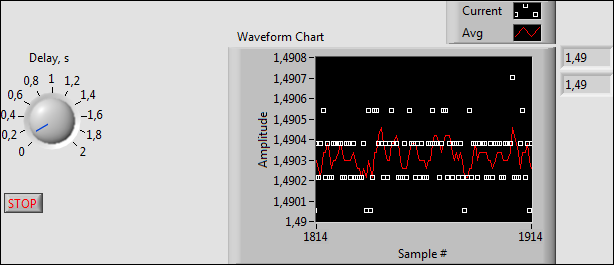
\includegraphics[width=\linewidth]{image/av_vi}
	\caption{Передняя панель Acquire Voltage}\label{img:av_vi}
\end{figure}


\begin{figure}[H]
	\centering		
	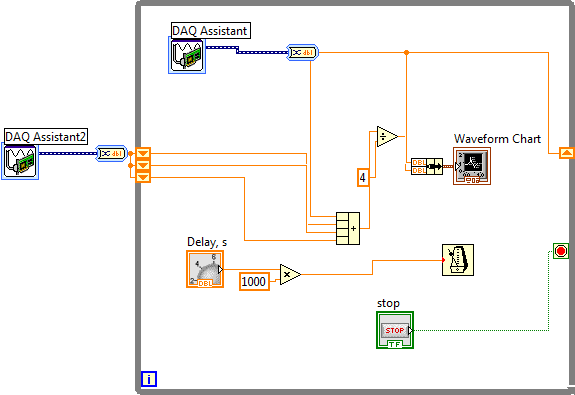
\includegraphics[width=\linewidth]{image/av_schema}
	\caption{Блок-схема Acquire Voltage}\label{img:av_schema}
\end{figure}

\subsection{Виртуальный прибор выполнения многократных измерений }

Краткое описание ВП Voltage Multiple Measurements.vi (ЛР 5, упр.5) со ссылками на рисунки передней панели и блок схемы. Рисунки передней панели и блок схемы. Описание не должно дублировать текст МУ.

\subsection{Some text}
Разделы с кратким описанием ВП Grubbs\_Test.vi или Outlier Test.vi (ЛР 6), mult\_process.vi (ЛР 7) со ссылками на рисунки передних панелей и блок-схем. Рисунки передних панелей и блок-схем. Можно приводить не все кейсы, а только те, на которых выполняется основная часть обработки. Описание не должно дублировать текст МУ 

\section{ПОРЯДОК ВЫПОЛНЕНИЯ РАБОТЫ}
\begin{enumerate}
\item 	Построение ВП для сбора и визуализации данных на основе Express-VI DAQ Assistant.
 Выполнение сбора и визуализации данных. 
 Исследование режимов отображения данных на диаграмме Waveform Chart. 
 Экспорт измеренных значений (таблица 1).
\item 	Построение ВП для выполнения и сохранения результатов многократных измерений.
 Выполнение многократных измерений, сохранение полученных результатов (таблица 2).
\item 	Построение ВП для проверки результатов измерений на наличие промахов. 
Проверка тестовой выборки (таблица 3.1), проверка результатов измерений (таблица  3.2).
\item 	Построение ВП для обработки результатов многократных измерений. 
Обработка тестовой выборки (таблица 4.1), результатов измерений (таблица 4.2).
\end{enumerate}

\section{ РЕЗУЛЬТАТЫ ИЗМЕРЕНИЙ И ВЫЧИСЛЕНИЙ}

\subsection{Результаты сбора данных}
Таблица и график с результатами измерений, полученные с помо-щью Acquire Voltage.vi (ЛР 5). 
Таблица 1
\subsection{Результаты многократных измерений}

Таблица с результатами измерений, полученных с помощью Voltage Multiple Measurements.vi (ЛР 6). Также записать максимальное, мини-мальное и среднее значения. 
Таблица 2
\subsection{Результаты проверки на промахи по критерию Граббса}

\section{ВЫВОДЫ ПО РАБОТЕ}
\end{document} % конец документа